\label{results:umbrella}
The basic patch is the main binding site of FAK to \pip{} and the membrane. The fact that the falling of FAK was only observed in \martini{} suggest that this binding is underestimated in the coarse-grained force field. Therefore, we calculated the free energy profile for \martini{} and compared it to equivalent simulations in \charmm{}. In the following, a short report on the results is given.\\
\\
The profiles are obtained from setup 2. The reaction coordinate is the z component of the COM distance between \pip{} and the protein fragment. For each forcefield, \charmm{}, \martini{} and \martini{} with PW, the average profile out of the five copies together with the standard deviation can be found in \autoref{umbrella:profiles}. The free energy profiles were shifted to be zero on average in the range $6\,\si{\nano\metre} \le z \le 7\,\si{\nano\metre}$.\\
%
%
%
% TODO: make c small in plot! --> not in GROMACS WHAM
\begin{figure}[hb]
	\centering
	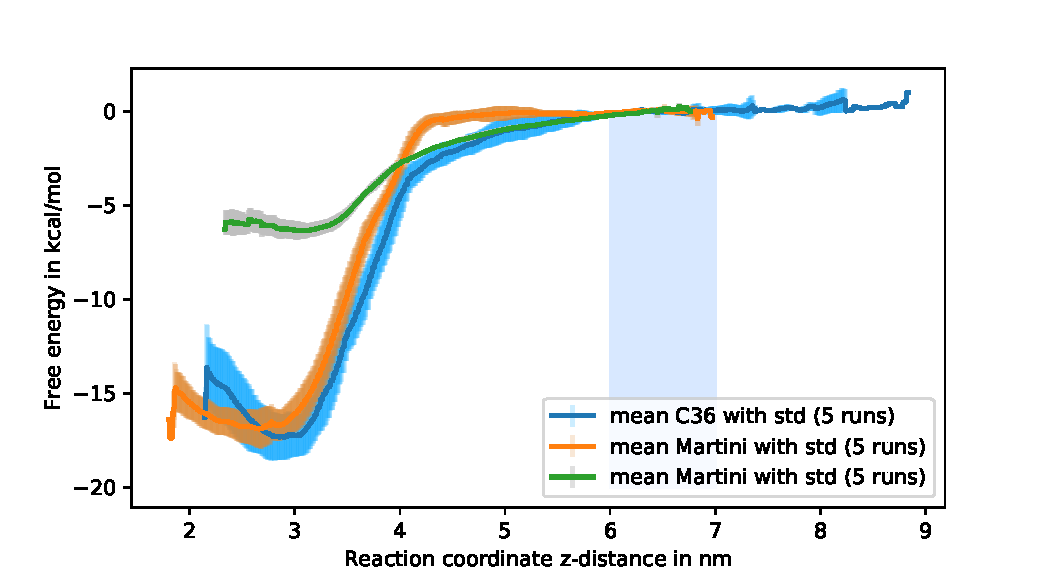
\includegraphics[width=.8\textwidth]{figures/results/umbrella}
	\nicecaption{Free energy profile of basic patch}{For each forcefield the average and standard deviation of the five copies is presented. All profiles are shifted to be zero in the blue region.}
	\label{umbrella:profiles}
\end{figure}
%
%
%
\\
Both force fields, \charmm{} and \martini{}, show a similar energy depth of $\approx 17 \si{\kilo Cal/\mole}$ and a similar slope between $3\,\si{\nano\metre} \le z \le 4\,\si{\nano\metre}$. The slight underestimation of the \martini{}-profile can be attributed to the proposed underestimation of electrostatic forces due to the non-polar water beads (see \autoref{subsub:coarsegraining}). However, the distance between profiles is smaller than the statistical error and not significant. The difference in the range $4\,\si{\nano\metre} \le z \le 6\,\si{\nano\metre}$ originates from the different treatment of long-range electrostatics: whereas \martini{} uses a cut-off radius, \charmm{} uses PME.\\
Also \martini{} with PW uses PME for long-range electrostatic interactions, and indeed it fits much better to the \charmm{} profile for larger distances. However, the binding strength is crucially underestimated in Martini with PW.\\
The extent to which \martini{} reproduces the results from all-atom simulations is remarkable, even though the parameters for \martini{} were obtained from free energy calculations (see \autoref{subsub:coarsegraining}).\\
\\
In the used starting configurations, the proteins are already bound to \pip{}. Therefore, a correct binding strength and the shape near the minimum is of larger interest than a correct sampling of farther distances. In addition, \martini{} with PW required a much higher computational effort. Hence, we consider only the standard water model in the following simulations.
